% Options for packages loaded elsewhere
\PassOptionsToPackage{unicode}{hyperref}
\PassOptionsToPackage{hyphens}{url}
%
\documentclass[
  12pt,
]{article}
\usepackage{lmodern}
\usepackage{amsmath}
\usepackage{ifxetex,ifluatex}
\ifnum 0\ifxetex 1\fi\ifluatex 1\fi=0 % if pdftex
  \usepackage[T1]{fontenc}
  \usepackage[utf8]{inputenc}
  \usepackage{textcomp} % provide euro and other symbols
  \usepackage{amssymb}
\else % if luatex or xetex
  \usepackage{unicode-math}
  \defaultfontfeatures{Scale=MatchLowercase}
  \defaultfontfeatures[\rmfamily]{Ligatures=TeX,Scale=1}
  \setmainfont[]{Times New Roman}
\fi
% Use upquote if available, for straight quotes in verbatim environments
\IfFileExists{upquote.sty}{\usepackage{upquote}}{}
\IfFileExists{microtype.sty}{% use microtype if available
  \usepackage[]{microtype}
  \UseMicrotypeSet[protrusion]{basicmath} % disable protrusion for tt fonts
}{}
\makeatletter
\@ifundefined{KOMAClassName}{% if non-KOMA class
  \IfFileExists{parskip.sty}{%
    \usepackage{parskip}
  }{% else
    \setlength{\parindent}{0pt}
    \setlength{\parskip}{6pt plus 2pt minus 1pt}}
}{% if KOMA class
  \KOMAoptions{parskip=half}}
\makeatother
\usepackage{xcolor}
\IfFileExists{xurl.sty}{\usepackage{xurl}}{} % add URL line breaks if available
\IfFileExists{bookmark.sty}{\usepackage{bookmark}}{\usepackage{hyperref}}
\hypersetup{
  pdftitle={Insert title of project here},
  pdfauthor={Zoe Wong, Molly Bruce},
  hidelinks,
  pdfcreator={LaTeX via pandoc}}
\urlstyle{same} % disable monospaced font for URLs
\usepackage[margin=2.54cm]{geometry}
\usepackage{longtable,booktabs}
\usepackage{calc} % for calculating minipage widths
% Correct order of tables after \paragraph or \subparagraph
\usepackage{etoolbox}
\makeatletter
\patchcmd\longtable{\par}{\if@noskipsec\mbox{}\fi\par}{}{}
\makeatother
% Allow footnotes in longtable head/foot
\IfFileExists{footnotehyper.sty}{\usepackage{footnotehyper}}{\usepackage{footnote}}
\makesavenoteenv{longtable}
\usepackage{graphicx}
\makeatletter
\def\maxwidth{\ifdim\Gin@nat@width>\linewidth\linewidth\else\Gin@nat@width\fi}
\def\maxheight{\ifdim\Gin@nat@height>\textheight\textheight\else\Gin@nat@height\fi}
\makeatother
% Scale images if necessary, so that they will not overflow the page
% margins by default, and it is still possible to overwrite the defaults
% using explicit options in \includegraphics[width, height, ...]{}
\setkeys{Gin}{width=\maxwidth,height=\maxheight,keepaspectratio}
% Set default figure placement to htbp
\makeatletter
\def\fps@figure{htbp}
\makeatother
\setlength{\emergencystretch}{3em} % prevent overfull lines
\providecommand{\tightlist}{%
  \setlength{\itemsep}{0pt}\setlength{\parskip}{0pt}}
\setcounter{secnumdepth}{5}
\ifluatex
  \usepackage{selnolig}  % disable illegal ligatures
\fi

\title{Insert title of project here}
\usepackage{etoolbox}
\makeatletter
\providecommand{\subtitle}[1]{% add subtitle to \maketitle
  \apptocmd{\@title}{\par {\large #1 \par}}{}{}
}
\makeatother
\subtitle{Web address for GitHub repository}
\author{Zoe Wong, Molly Bruce}
\date{}

\begin{document}
\maketitle

\newpage
\tableofcontents 
\newpage
\listoftables 
\newpage
\listoffigures 
\newpage

\hypertarget{rationale-and-research-questions}{%
\section{Rationale and Research
Questions}\label{rationale-and-research-questions}}

\hypertarget{research-questions}{%
\subsection{Research Questions}\label{research-questions}}

\begin{enumerate}
\def\labelenumi{\arabic{enumi}.}
\tightlist
\item
  When consumers buy seafood, which species do they prefer? Do they
  prefer wild or farmed fish?
\item
  What qualities do consumers associate with wild vs.~farmed seafood?
  What qualities do they value in seafood?
\item
  Are seafood values predicted by demographic variables such as age or
  education level?
\end{enumerate}

\newpage

\hypertarget{dataset-information}{%
\section{Dataset Information}\label{dataset-information}}

\hypertarget{description-of-the-data}{%
\subsection{Description of the Data}\label{description-of-the-data}}

Our data were obtained from a social science survey conducted by a
multi-university team of researchers, including the Murray lab at Duke
University. The survey was conducted in the summer of 2020 via Qualtrics
and targeted North Carolina residents from across the state.

The survey asked respondents a total of 37 questions. The question
topics can be broken down into the following categories: eating habits
for 8 types of seafood, what qualities respondents associate with
seafood, attitudes about mariculture, attitudes about North Carolina
seafood versus commercial fishing, respondents' involvement with seafood
production, and demographic indicators. This study focuses on questions
about eating habits, what qualities are associated with seafood, and
demographic indicators.

Respondents answered each question by selecting one option from a menu
of choices; the number of choices available depended on the question.
The dataset contained responses from 1436 participants.

\hypertarget{data-wrangling}{%
\subsection{Data Wrangling}\label{data-wrangling}}

For each analysis, we created a new dataset containing only the relevant
columns. For each category within the survey question, we then created a
table with the frequency of each questions response. For example, one
question asked respondents to rate how often they ate each of 8 types of
seafood; respondents could choose from 7 responses for each seafood
type. To wrangle this data, we created a dataframe for each type of
seafood, for a total of 8 dataframes, each of which contained a column
with the response choices and a column with the number of respondents
that chose each response. Because the response choices were only
represented by a number in the raw data, we renamed the response column
with the meaning of each number for greater clarity. We repeated this
process for the first two research questions (how often participants eat
each type of seafood, whether participants prefer each type wild or
farmed, whether participants associate each quality with wild or farmed
seafood).

For the fourth research question, we created a dataframe with responses
to a question about how important each of 11 qualities was when
respondents were buying seafood. We then renamed the columns and removed
rows with alternate responses to demographic variables, such as ``prefer
not to answer.''

\hypertarget{data-structure-consumer-preferences}{%
\subsection{Data Structure: Consumer
preferences}\label{data-structure-consumer-preferences}}

\begin{longtable}[]{@{}llll@{}}
\toprule
\begin{minipage}[b]{(\columnwidth - 3\tabcolsep) * \real{0.26}}\raggedright
Research Question\strut
\end{minipage} &
\begin{minipage}[b]{(\columnwidth - 3\tabcolsep) * \real{0.31}}\raggedright
Survey Question\strut
\end{minipage} &
\begin{minipage}[b]{(\columnwidth - 3\tabcolsep) * \real{0.19}}\raggedright
Iterations\strut
\end{minipage} &
\begin{minipage}[b]{(\columnwidth - 3\tabcolsep) * \real{0.24}}\raggedright
Response choices\strut
\end{minipage}\tabularnewline
\midrule
\endhead
\begin{minipage}[t]{(\columnwidth - 3\tabcolsep) * \real{0.26}}\raggedright
1. When consumers buy seafood, which species do they prefer?\strut
\end{minipage} &
\begin{minipage}[t]{(\columnwidth - 3\tabcolsep) * \real{0.31}}\raggedright
In the past year, how often did you eat the following type of
seafood?\strut
\end{minipage} &
\begin{minipage}[t]{(\columnwidth - 3\tabcolsep) * \real{0.19}}\raggedright
Tuna, Shrimp, Salmon, Flounder, Blue Crab, Clams, Mullet, Oysters
(8)\strut
\end{minipage} &
\begin{minipage}[t]{(\columnwidth - 3\tabcolsep) * \real{0.24}}\raggedright
0 = Never, 1 = Once in the past year, 2 = A few times in the past year,
3 = Once a month, 4 = A few times every month, 5 = Once a week, 6 = More
than once a week\strut
\end{minipage}\tabularnewline
\begin{minipage}[t]{(\columnwidth - 3\tabcolsep) * \real{0.26}}\raggedright
1. Do consumers prefer wild or farmed fish?\strut
\end{minipage} &
\begin{minipage}[t]{(\columnwidth - 3\tabcolsep) * \real{0.31}}\raggedright
Between wild-caught and farmed versions of the same seafood species,
which do you prefer to eat?\strut
\end{minipage} &
\begin{minipage}[t]{(\columnwidth - 3\tabcolsep) * \real{0.19}}\raggedright
Tuna, Shrimp, Salmon, Flounder, Blue Crab, Clams, Mullet, Oysters
(8)\strut
\end{minipage} &
\begin{minipage}[t]{(\columnwidth - 3\tabcolsep) * \real{0.24}}\raggedright
1 = Strongly prefer wild-caught, 2 = Slightly prefer wild-caught, 3 = No
preference, 4 = Slightly prefer farmed, 5 = Strongly prefer farmed, 6 =
I don't know\strut
\end{minipage}\tabularnewline
\begin{minipage}[t]{(\columnwidth - 3\tabcolsep) * \real{0.26}}\raggedright
2. What qualities do consumers associate with wild vs.~farmed
seafood?\strut
\end{minipage} &
\begin{minipage}[t]{(\columnwidth - 3\tabcolsep) * \real{0.31}}\raggedright
How do you associate the following qualities with different types of
seafood (farmed and wild-caught)?\strut
\end{minipage} &
\begin{minipage}[t]{(\columnwidth - 3\tabcolsep) * \real{0.19}}\raggedright
Healthy, Local, Safe, Tasty, Affordable, Sustainable, Fresh, Easy
Access, Local Culture, Local Economies, Local Environment (11)\strut
\end{minipage} &
\begin{minipage}[t]{(\columnwidth - 3\tabcolsep) * \real{0.24}}\raggedright
1 = More associated with wild-caught, 2 = Associated equally with
wild-caught and farmed, 3 = More associated with farmed, 4 = Associated
with neither wild-caught or farmed, 5 = I don't know\strut
\end{minipage}\tabularnewline
\begin{minipage}[t]{(\columnwidth - 3\tabcolsep) * \real{0.26}}\raggedright
2. What qualities do consumers value in seafood?\strut
\end{minipage} &
\begin{minipage}[t]{(\columnwidth - 3\tabcolsep) * \real{0.31}}\raggedright
When you are buying seafood, how important are the following qualities
to you?\strut
\end{minipage} &
\begin{minipage}[t]{(\columnwidth - 3\tabcolsep) * \real{0.19}}\raggedright
Healthy, Local, Safe, Tasty, Affordable, Sustainable, Fresh, Easy
Access, Local Culture, Local Economies, Local Environment (11)\strut
\end{minipage} &
\begin{minipage}[t]{(\columnwidth - 3\tabcolsep) * \real{0.24}}\raggedright
1 = Not at all important, 2 = Slightly important, 3 = Moderately
important, 4 = Very important, 5 = Extremely important\strut
\end{minipage}\tabularnewline
\bottomrule
\end{longtable}

\hypertarget{data-structure-demographics}{%
\subsection{Data structure:
Demographics}\label{data-structure-demographics}}

\begin{longtable}[]{@{}lll@{}}
\toprule
\begin{minipage}[b]{(\columnwidth - 2\tabcolsep) * \real{0.23}}\raggedright
Demographic Category\strut
\end{minipage} &
\begin{minipage}[b]{(\columnwidth - 2\tabcolsep) * \real{0.36}}\raggedright
Response choices\strut
\end{minipage} &
\begin{minipage}[b]{(\columnwidth - 2\tabcolsep) * \real{0.41}}\raggedright
Counts\strut
\end{minipage}\tabularnewline
\midrule
\endhead
\begin{minipage}[t]{(\columnwidth - 2\tabcolsep) * \real{0.23}}\raggedright
Age\strut
\end{minipage} &
\begin{minipage}[t]{(\columnwidth - 2\tabcolsep) * \real{0.36}}\raggedright
1=19 or younger ~2=20-29 ~3=30-39 ~4=40-49 ~5=50-59 ~6=60-69, 7=70 or
older, 8=Prefer not to answer\strut
\end{minipage} &
\begin{minipage}[t]{(\columnwidth - 2\tabcolsep) * \real{0.41}}\raggedright
\strut
\end{minipage}\tabularnewline
\begin{minipage}[t]{(\columnwidth - 2\tabcolsep) * \real{0.23}}\raggedright
Gender\strut
\end{minipage} &
\begin{minipage}[t]{(\columnwidth - 2\tabcolsep) * \real{0.36}}\raggedright
\strut
\end{minipage} &
\begin{minipage}[t]{(\columnwidth - 2\tabcolsep) * \real{0.41}}\raggedright
\strut
\end{minipage}\tabularnewline
\begin{minipage}[t]{(\columnwidth - 2\tabcolsep) * \real{0.23}}\raggedright
3. Are seafood values predicted by demographic variables such as age or
education level?\strut
\end{minipage} &
\begin{minipage}[t]{(\columnwidth - 2\tabcolsep) * \real{0.36}}\raggedright
\strut
\end{minipage} &
\begin{minipage}[t]{(\columnwidth - 2\tabcolsep) * \real{0.41}}\raggedright
Age, Gender, Education Level, Political Party, Race, Income Level
(6)\strut
\end{minipage}\tabularnewline
\bottomrule
\end{longtable}

\newpage

\hypertarget{exploratory-analysis}{%
\section{Exploratory Analysis}\label{exploratory-analysis}}

\begin{itemize}
\tightlist
\item
  frequency general?
\item
  map of counties where respondents live?
\end{itemize}

\newpage

\hypertarget{analysis}{%
\section{Analysis}\label{analysis}}

\hypertarget{question-1-when-consumers-buy-seafood-which-species-do-they-prefer}{%
\subsection{Question 1: When consumers buy seafood, which species do
they
prefer?}\label{question-1-when-consumers-buy-seafood-which-species-do-they-prefer}}

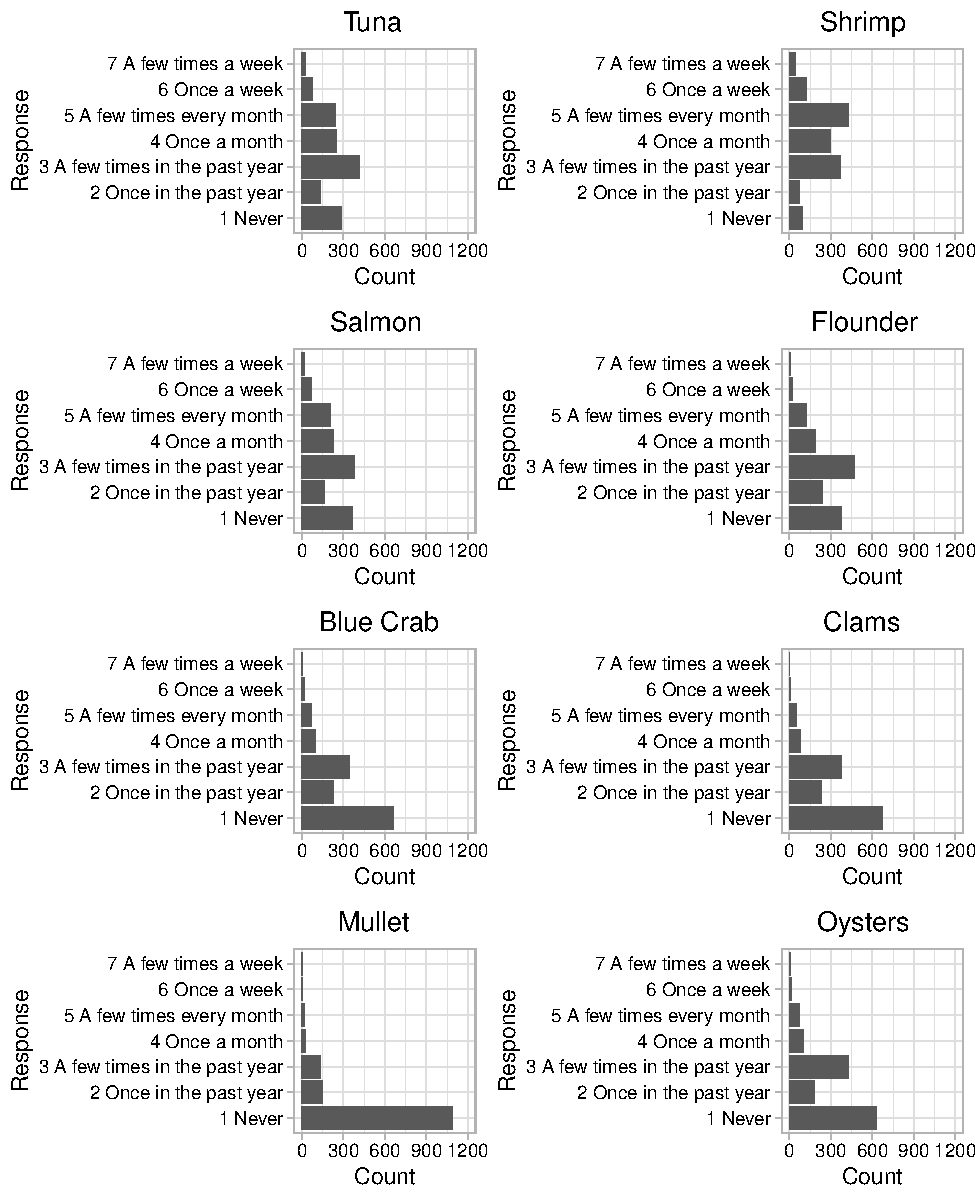
\includegraphics{Final_rmd_files/figure-latex/frequency-1.pdf}

{[}explanation of frequency findings. also add fig.cap above{]}

\hypertarget{question-1a-do-consumers-prefer-wild-or-farmed-fish}{%
\subsubsection{Question 1a: Do consumers prefer wild or farmed
fish?}\label{question-1a-do-consumers-prefer-wild-or-farmed-fish}}

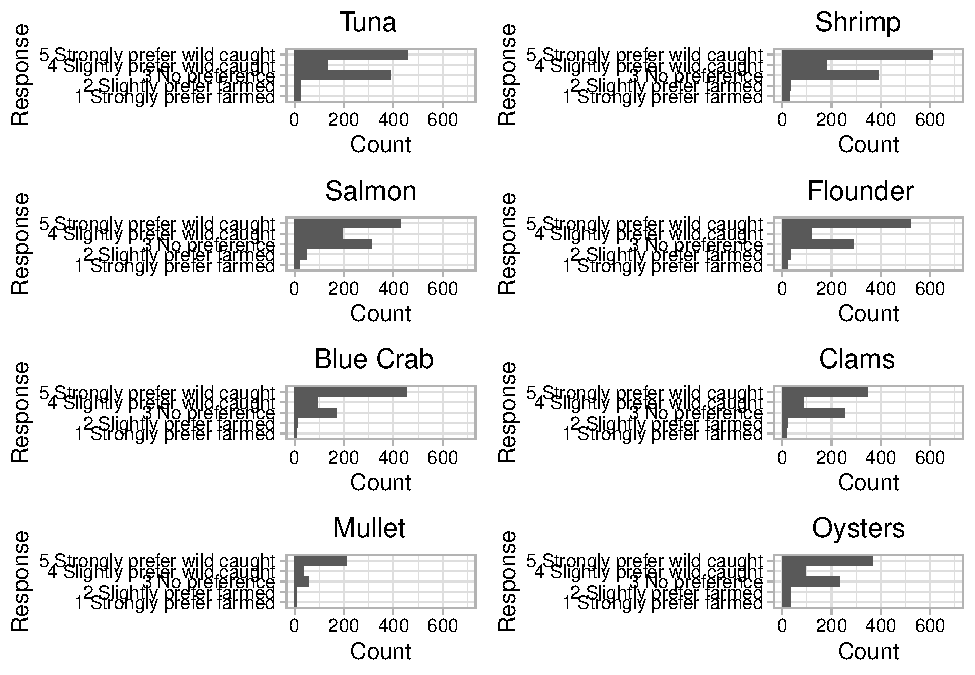
\includegraphics{Final_rmd_files/figure-latex/preference-1.pdf}

{[}explanation of findings. also add fig.cap above{]}

\hypertarget{question-2-what-qualities-do-consumers-associate-with-seafood-what-qualities-do-they-value-in-seafood}{%
\subsection{Question 2: What qualities do consumers associate with
seafood? What qualities do they value in
seafood?}\label{question-2-what-qualities-do-consumers-associate-with-seafood-what-qualities-do-they-value-in-seafood}}

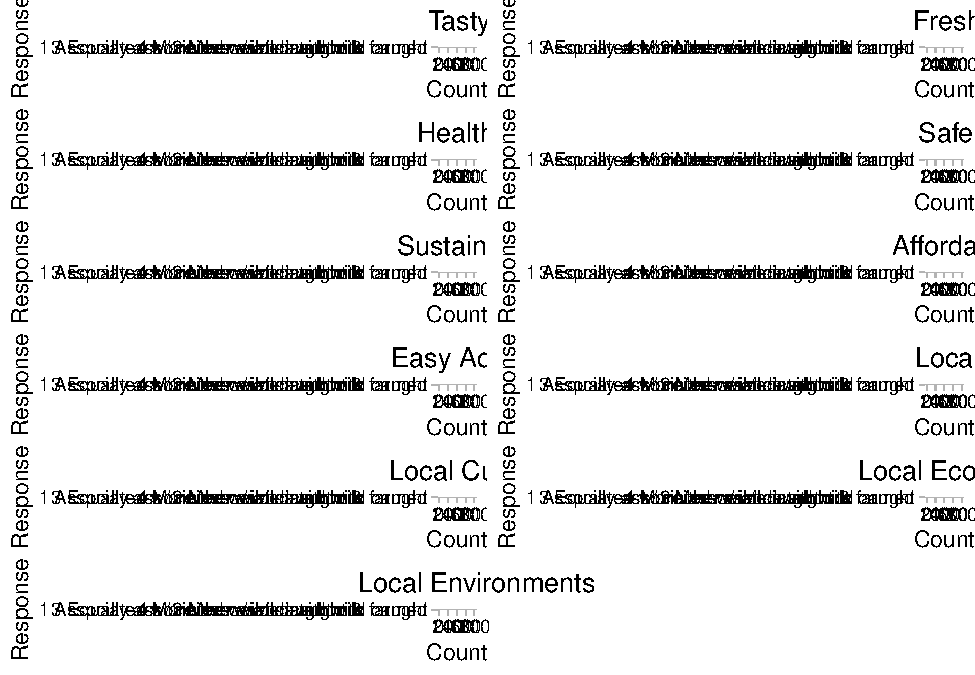
\includegraphics{Final_rmd_files/figure-latex/qualities-1.pdf}

{[}explanation of findings. also add fig.cap above{]}

\hypertarget{question-3-are-seafood-values-predicted-by-demographic-variables-such-as-age-or-education-level}{%
\subsection{Question 3: Are seafood values predicted by demographic
variables such as age or education
level?}\label{question-3-are-seafood-values-predicted-by-demographic-variables-such-as-age-or-education-level}}

\newpage

\hypertarget{summary-and-conclusions}{%
\section{Summary and Conclusions}\label{summary-and-conclusions}}

\newpage

\hypertarget{references}{%
\section{References}\label{references}}

\textless add references here if relevant, otherwise delete this
section\textgreater{}

\end{document}
